%----------------------------------------------------------------------
% 實驗設計分析
%----------------------------------------------------------------------

\chapter{Evaluation}\label{sec:evalutaion}
\section{Experiment }\label{sec:3-experiment}
\subsection{Experiment Setup}\label{sec:3-setup}
To test the performance of the algorithm, 3 specific scenarios were tested:
1. Control scenario, when object 1 (white) and object 2 (yellow) do not crosspath.
2. One object conceals another and continues their original trajectory after departing.
3. One object conceals another and changes trajectory when departing.
\begin{figure}[!htb]
    \centering
    \begin{subfigure}{0.25\linewidth}
        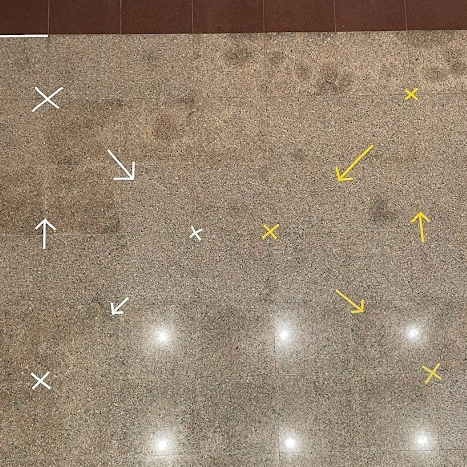
\includegraphics[width=5.5cm]{Figures/scenario_1_gt.png}
        \caption{scenario 1}
        \label{subfig:scenario1gt}
    \end{subfigure}
    \hfill
    \begin{subfigure}{0.25\linewidth}
        \centering
        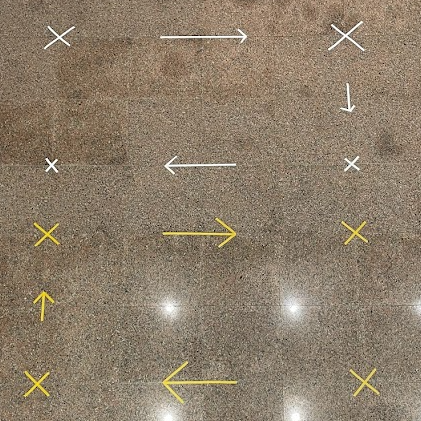
\includegraphics[width=5.5cm]{Figures/scenario_2_gt.png}
        \caption{scenario 2}
        \label{subfig:scenario2gt}
    \end{subfigure}
    \hfill
    \begin{subfigure}{0.25\linewidth}
        \centering
        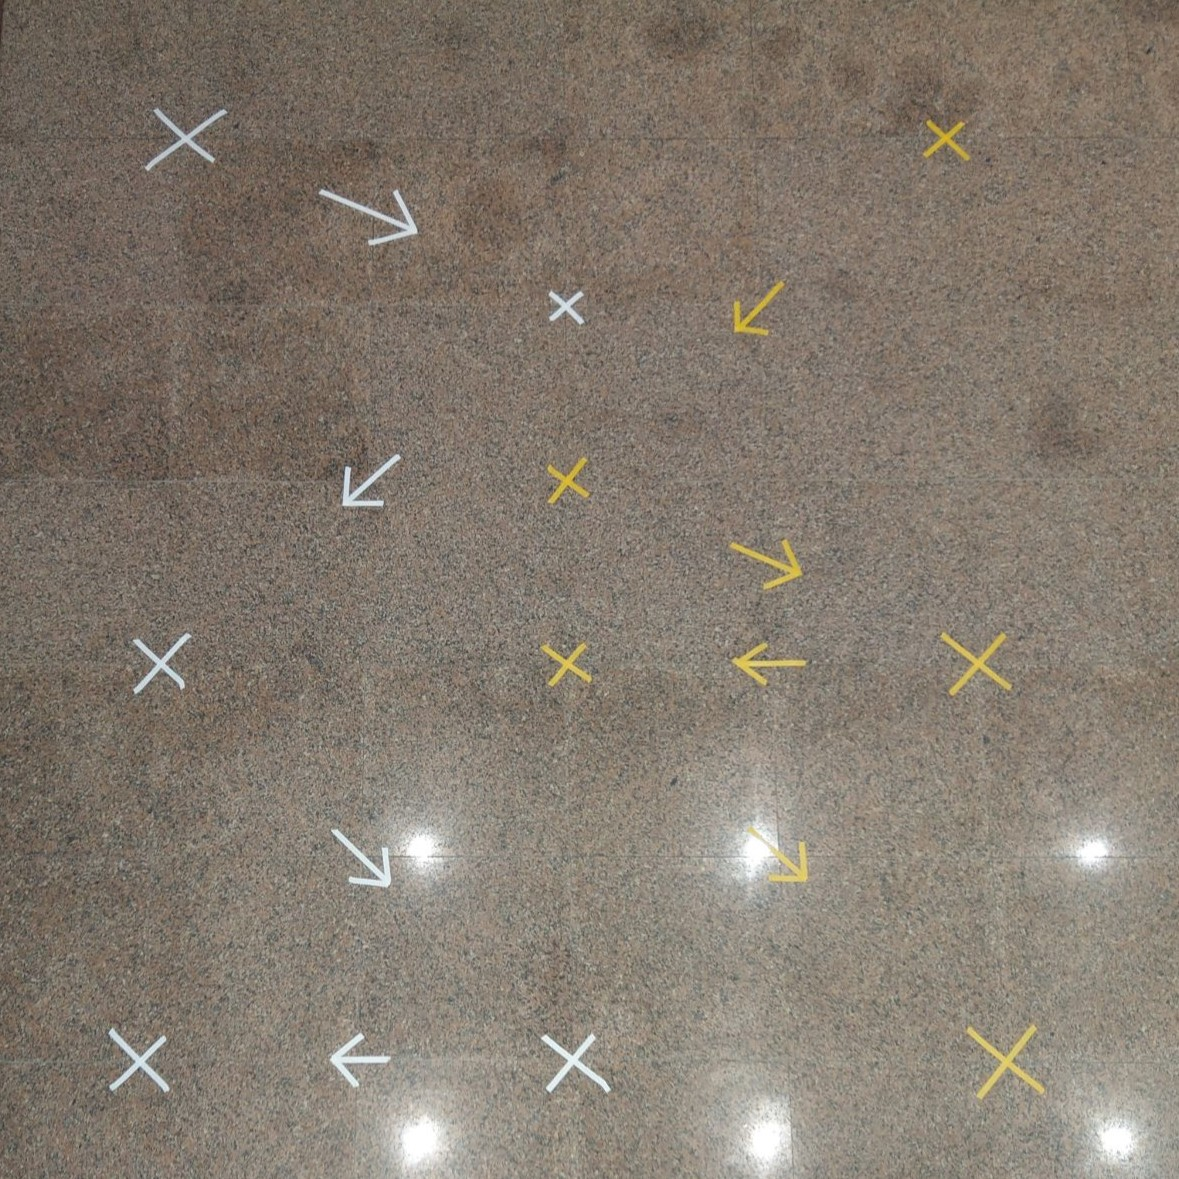
\includegraphics[width=5.5cm]{Figures/scenario_3_gt.jpg}
        \caption{scenario 3}
        \label{subfig:scenario3gt}
    \end{subfigure}

    \caption{Ground truth of multi-object tracking experiments}
    \label{fig:ground_truth}
\end{figure}

\subsection{Challenges to Overcome}\label{sec:3-challenge}
Blind spot of both sensors.
Challenges the algorithm to correctly predict objects when data is obstructed.

\begin{figure}[!htb]
    \centering
    \begin{subfigure}{0.3\linewidth}
        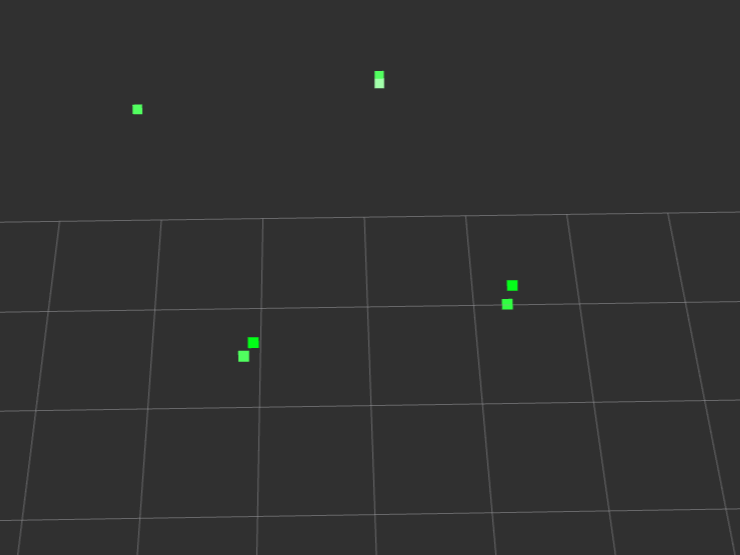
\includegraphics[width=7cm]{Figures/before_conceal_radar.png}
        \caption{Raw radar data}
        \label{subfig:before_conceal_radar_fig}
    \end{subfigure}
    \hspace{0.15\textwidth}
    %\hfill
    \begin{subfigure}{0.3\linewidth}
        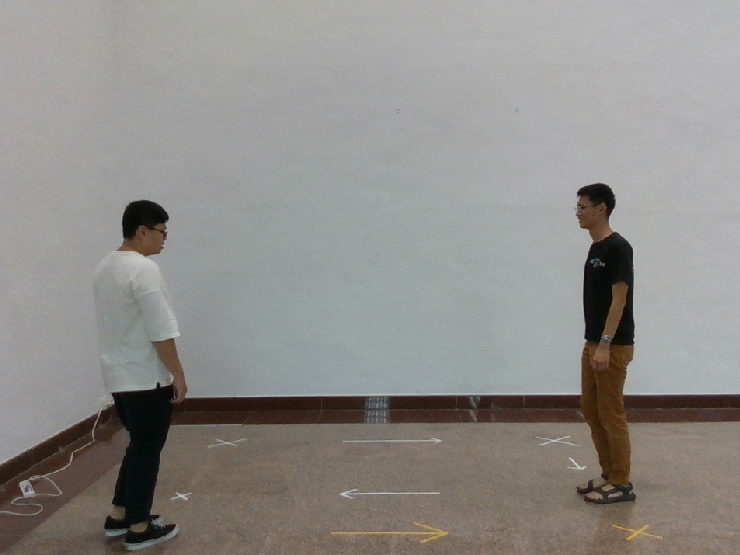
\includegraphics[width=7cm]{Figures/before_conceal_image.png}
        \caption{Image frame}
        \label{subfig:before_conceal_image_fig}
    \end{subfigure}

    \caption{Object 1 and object 2 before crossingpath}
    \label{fig:before_conceal_fig}
\end{figure}

From figure \ref*{fig:concealing_fig}\subref{subfig:concealing_radar_fig} can be seen that both object clusters disappear.



\begin{figure}[!htb]
    \centering
    \begin{subfigure}{0.3\linewidth}
        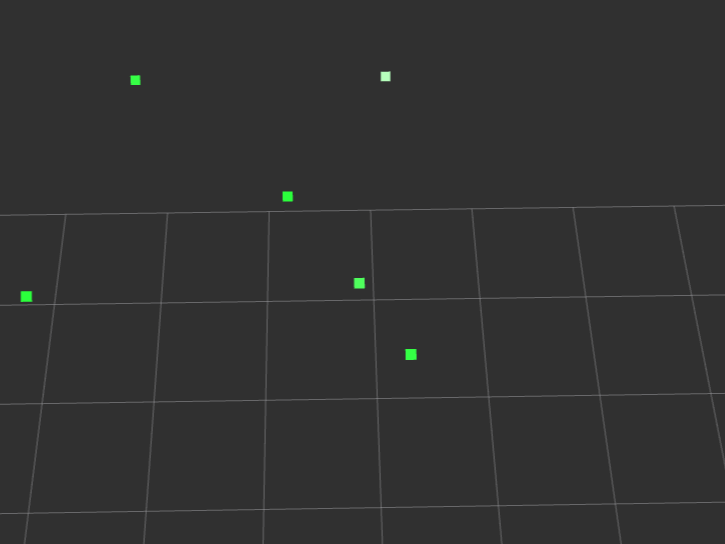
\includegraphics[width=7cm]{Figures/concealing_radar.png}
        \caption{Raw radar data}
        \label{subfig:concealing_radar_fig}
    \end{subfigure}
    \hspace{0.15\textwidth}
    %\hfill
    \begin{subfigure}{0.3\linewidth}
        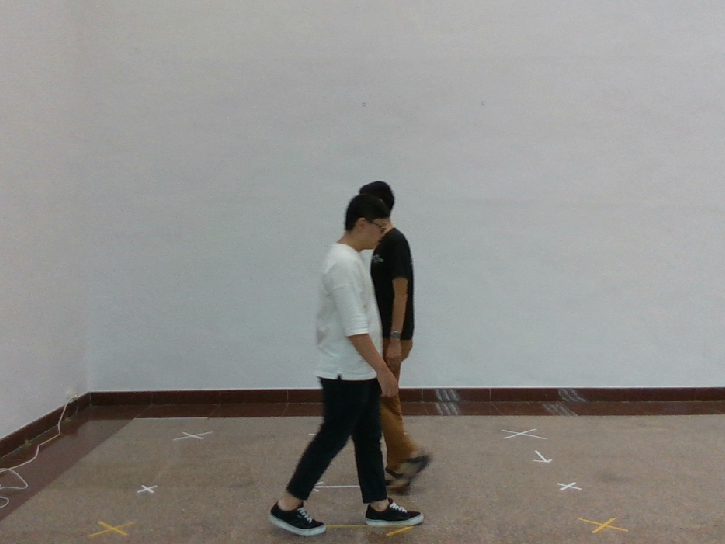
\includegraphics[width=7cm]{Figures/concealing_image.png}
        \caption{Image frame}
        \label{subfig:concealing_image_fig}
    \end{subfigure}

    \caption{Object 1 covers object 2}
    \label{fig:concealing_fig}
\end{figure}

\begin{figure}[!htb]
    \centering
    \begin{subfigure}{0.3\linewidth}
        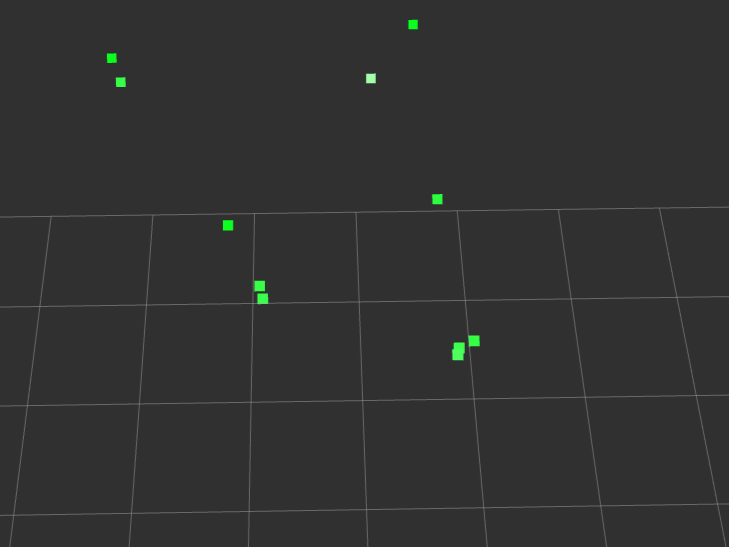
\includegraphics[width=7cm]{Figures/after_conceal_radar.png}
        \caption{Raw radar data}
        \label{subfig:after_conceal_radar_fig}
    \end{subfigure}
    \hspace{0.15\textwidth}
    %\hfill
    \begin{subfigure}{0.3\linewidth}
        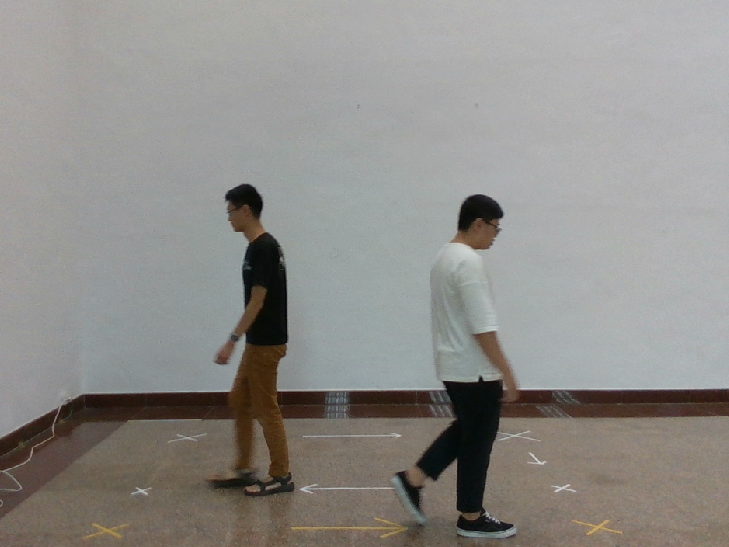
\includegraphics[width=7cm]{Figures/after_conceal_image.png}
        \caption{Image frame}
        \label{subfig:after_conceal_image_fig}
    \end{subfigure}

    \caption{Object 1 and object 2 seperates}
    \label{fig:after_conceal_fig}
\end{figure}





\vspace*{5cm}
\subsection{Experiment Result}\label{sec:3-exp_result}
\subsubsection{Scenario 1}\label{sec:3-exp_result1}
Scenario 1 is the control when object 1 and object 2 do not crosspath.
\href{https://drive.google.com/file/d/1SL30CC6EpyI4NLOcGnfALKAP44P82u9n/view?usp=sharing}{\color{blue}{Video click me}}
\begin{figure}[!htb]
    \centering
    \begin{subfigure}[b]{0.475\textwidth}%{0.25\linewidth}
        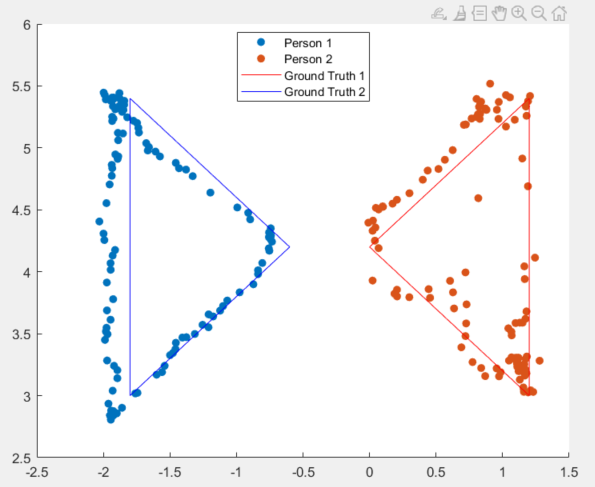
\includegraphics[width=7cm]{Figures/1_before.png}
        \caption{Only radar object tracking}
        \label{subfig:without_fusion_1}
    \end{subfigure}
    %\hspace{0.15\textwidth}
    \hfill
    \begin{subfigure}[b]{0.475\textwidth}%{0.25\linewidth}
        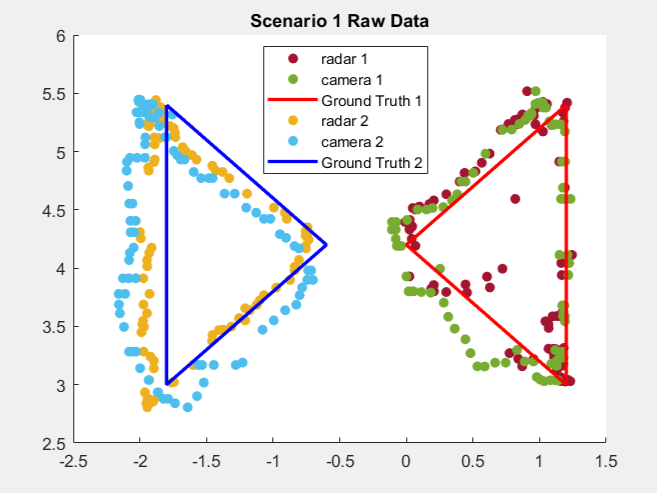
\includegraphics[width=7cm]{Figures/raw_scene1.png}
        \caption{Raw radar and image data after data association}
        \label{subfig:raw_fusion_1}
    \end{subfigure}
    %\hfill
    \vskip\baselineskip

    \begin{subfigure}[b]{0.475\textwidth}%{0.25\linewidth}
        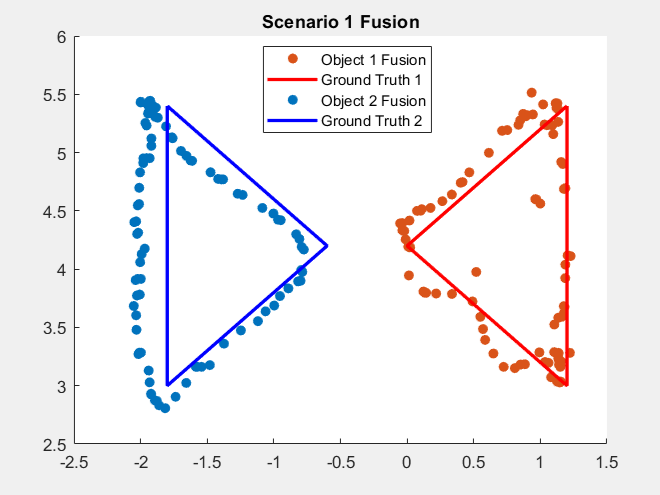
\includegraphics[width=7cm]{Figures/fusion_scene1.png}
        \caption{Fused data}
        \label{subfig:fusion_1}
    \end{subfigure}

    \begin{subfigure}[b]{0.475\textwidth}%{0.25\linewidth}
        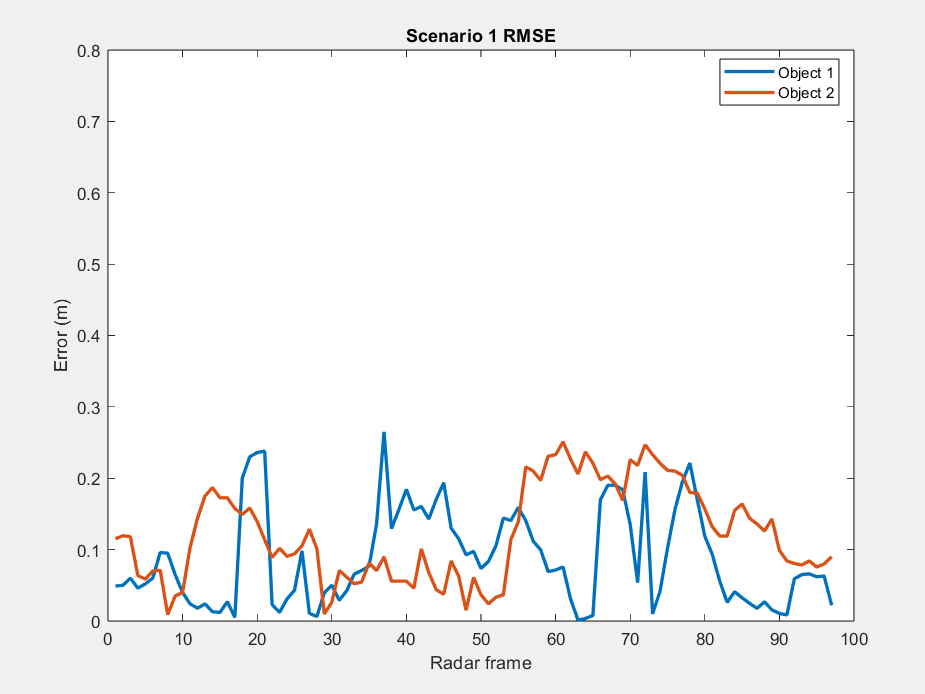
\includegraphics[width=7cm]{Figures/RMSE1.png}
        \caption{RMSE to ground truth}
        \label{subfig:RMSE_1}
    \end{subfigure}

    \caption{Scenario 1 multi-object tracking}
    \label{fig:scenario_result_1}
\end{figure}

\subsubsection{Scenario 2}\label{sec:3-exp_result2}
In scenario 2, object 1 crosses path with object 2 in a straight line horizontally.
After concealing object 2 from both camera and radar, both objects continue their original trajectory.
In figure \ref*{fig:scenario_result_2}\subref{subfig:without_fusion_2} can be seen that object 1 and object 2 switch places.
The algorithm is able to track and identify objects 1 and 2 correctly (figure \ref*{fig:scenario_result_2}\subref{subfig:with_fusion_2}).
\href{https://drive.google.com/file/d/1YnliV7YRzahYNpIehctzrNrf0Z0ZpIeY/view?usp=sharing}{\color{blue}{Video click me}}
\begin{figure}[!htb]
    \centering
    \begin{subfigure}[b]{0.475\textwidth}%{0.25\linewidth}
        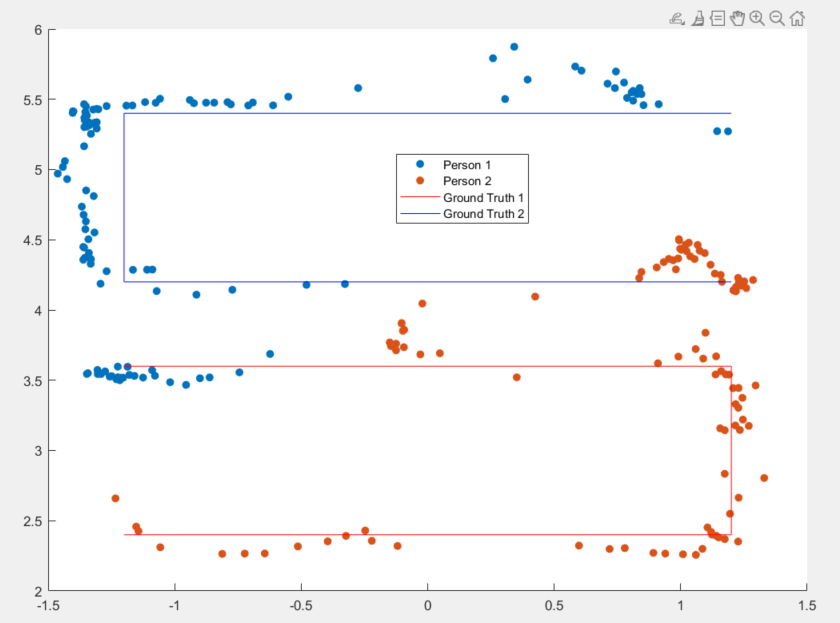
\includegraphics[width=7cm]{Figures/2_before.png}
        \caption{Only radar object tracking}
        \label{subfig:without_fusion_2}
    \end{subfigure}
    %\hspace{0.15\textwidth}
    \hfill
    \begin{subfigure}[b]{0.475\textwidth}%{0.25\linewidth}
        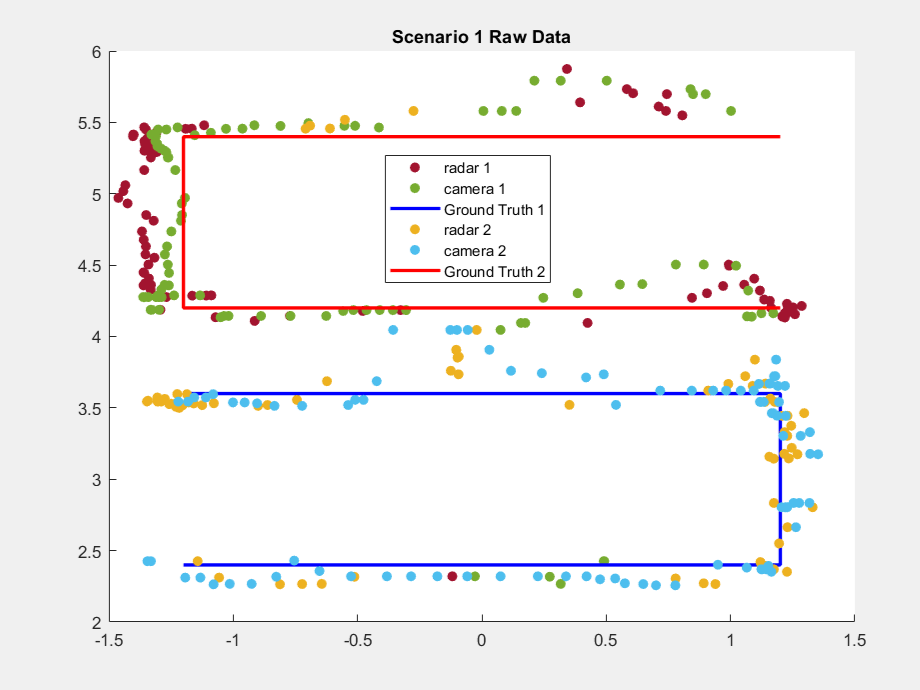
\includegraphics[width=7cm]{Figures/raw_scene2.png}
        \caption{Raw radar and image data after data association}
        \label{subfig:raw_fusion_2}
    \end{subfigure}
    %\hfill
    \vskip\baselineskip

    \begin{subfigure}[b]{0.475\textwidth}%{0.25\linewidth}
        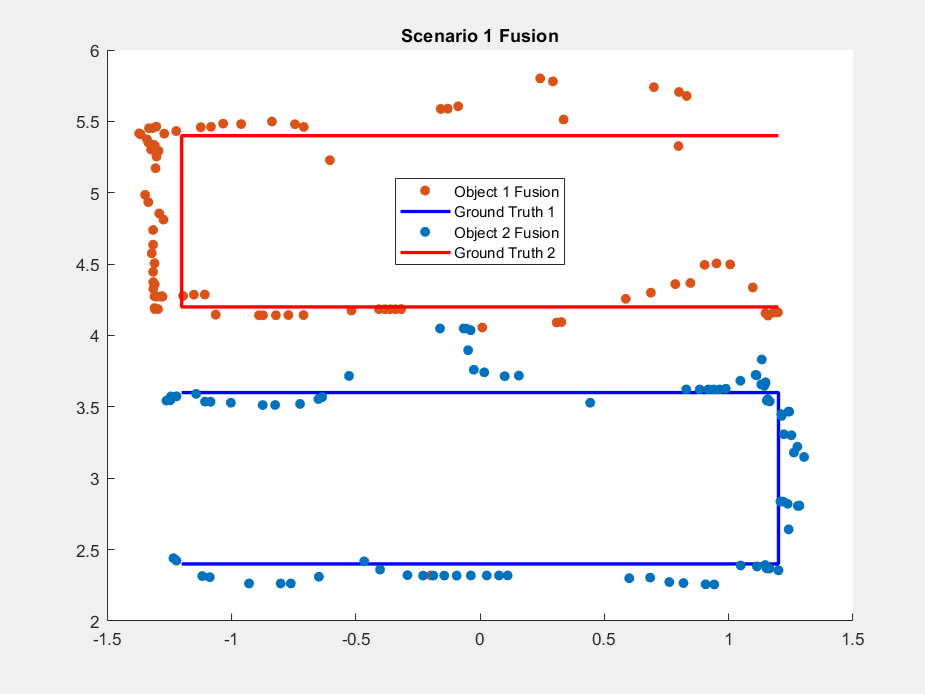
\includegraphics[width=7cm]{Figures/fusion_scene2.png}
        \caption{Fused data}
        \label{subfig:with_fusion_2}
    \end{subfigure}
    \begin{subfigure}[b]{0.475\textwidth}%{0.25\linewidth}
        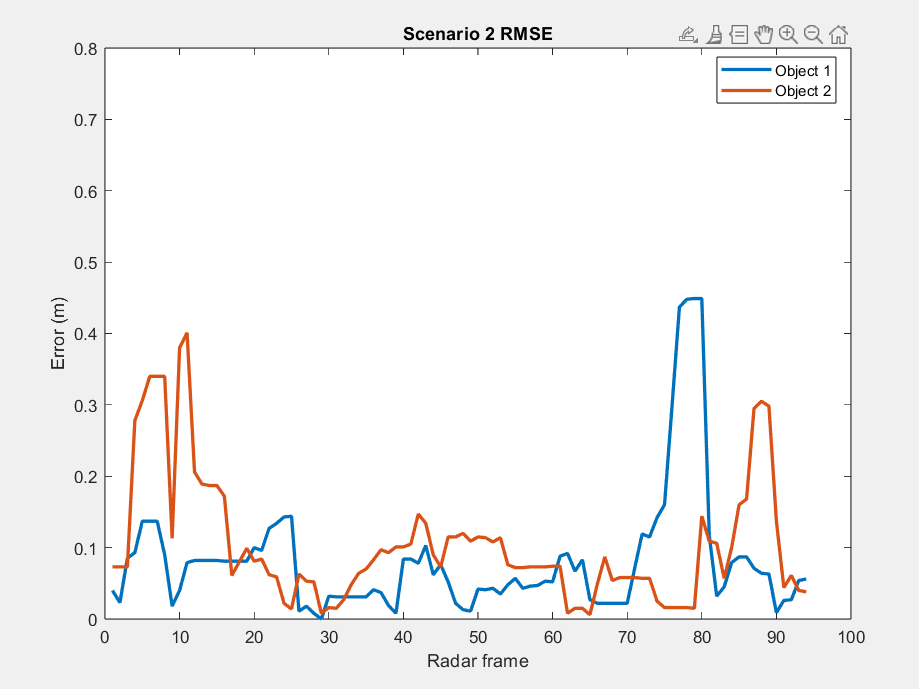
\includegraphics[width=7cm]{Figures/RMSE2.png}
        \caption{RMSE to ground truth}
        \label{subfig:RMSE_2}
    \end{subfigure}
    \caption{Scenario 2 multi-object tracking}
    \label{fig:scenario_result_2}
\end{figure}
\newpage
\subsubsection{Scenario 3}\label{sec:3-exp_result3}
In scenario 3, object 1 covers object 2, and in the next few frames, object 2 covers object 1.
In this scenario, both objects change trajectory when departing from each other.
In figure \ref*{fig:scenario_result_3}\subref{subfig:without_fusion_3} can be seen that object 1 and object 2 switch places.
The algorithm is able to track and identify objects 1 and 2 correctly (figure \ref*{fig:scenario_result_3}\subref{subfig:with_fusion_3}).
\href{https://drive.google.com/file/d/1bd92Bu6CJeL1QIIbBlW42cAozxEcis-d/view?usp=sharing}{\color{blue}{Video click me}}
\begin{figure}[!htb]
    \centering
    %\begin{adjustwidth}{-8em}{0em}
    \begin{subfigure}[b]{0.475\textwidth}%{0.25\linewidth}
        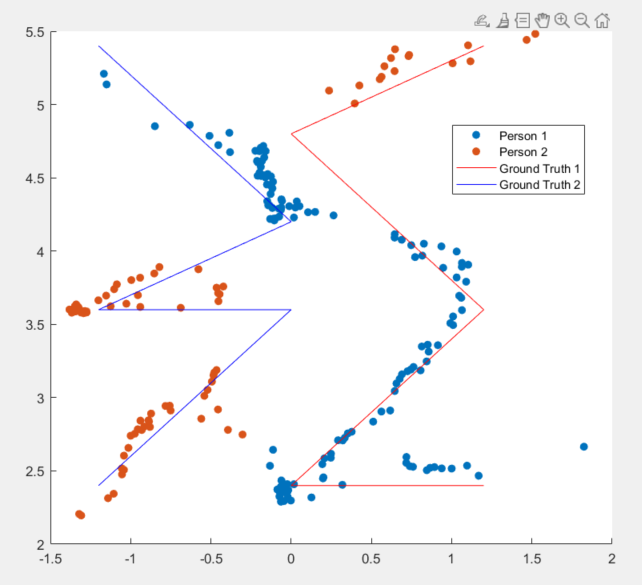
\includegraphics[width=7cm]{Figures/3_before.png}
        \caption{Only radar object tracking}
        \label{subfig:without_fusion_3}
    \end{subfigure}
    %\hspace{0.05\textwidth}
    \hfill
    \begin{subfigure}[b]{0.475\textwidth}%{0.25\linewidth}
        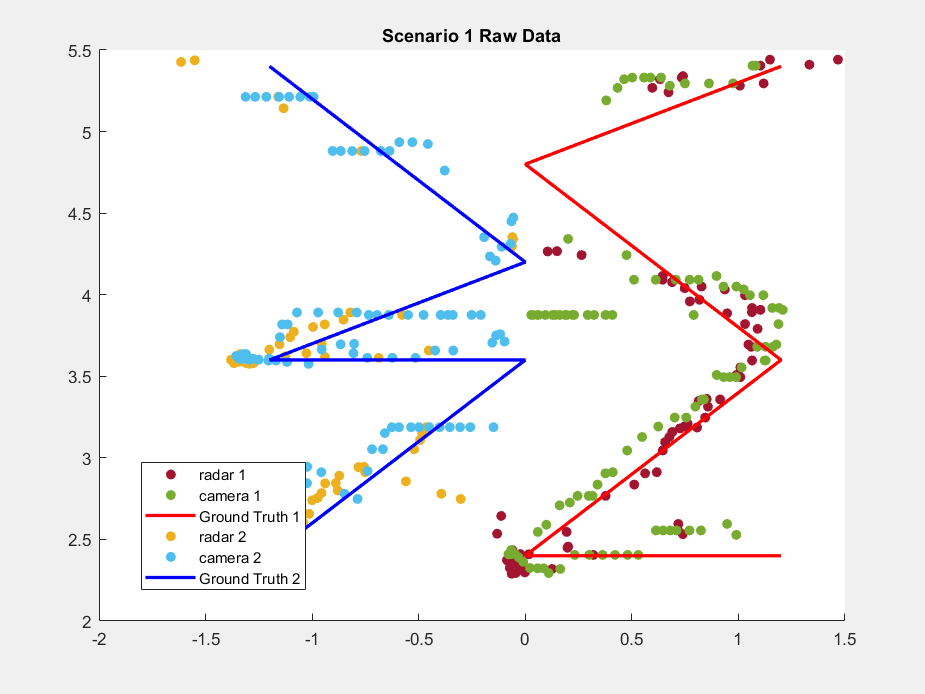
\includegraphics[width=7cm]{Figures/raw_scene3.png}
        \caption{Raw radar and image data after data association}
        \label{subfig:raw_fusion_3}
    \end{subfigure}
    \vskip\baselineskip
%\end{adjustwidth}
    %\hfill
    %\hspace{0.05\textwidth}

    \begin{subfigure}[b]{0.475\textwidth}%{0.25\linewidth}
        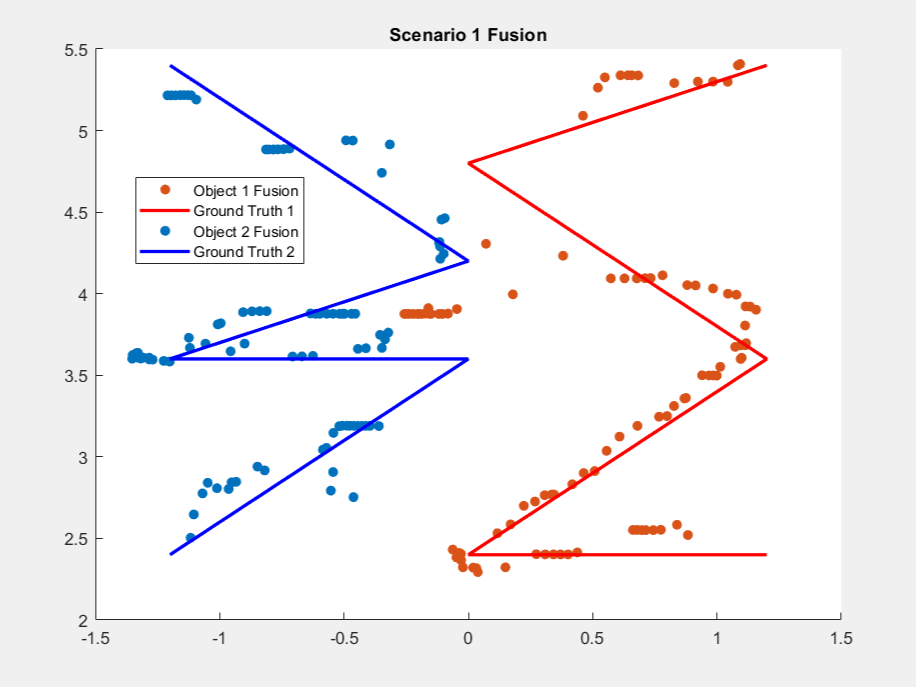
\includegraphics[width=7cm]{Figures/fusion_scene3.png}
        \caption{Fused data}
        \label{subfig:with_fusion_3}
    \end{subfigure}
    \begin{subfigure}[b]{0.475\textwidth}%{0.25\linewidth}
        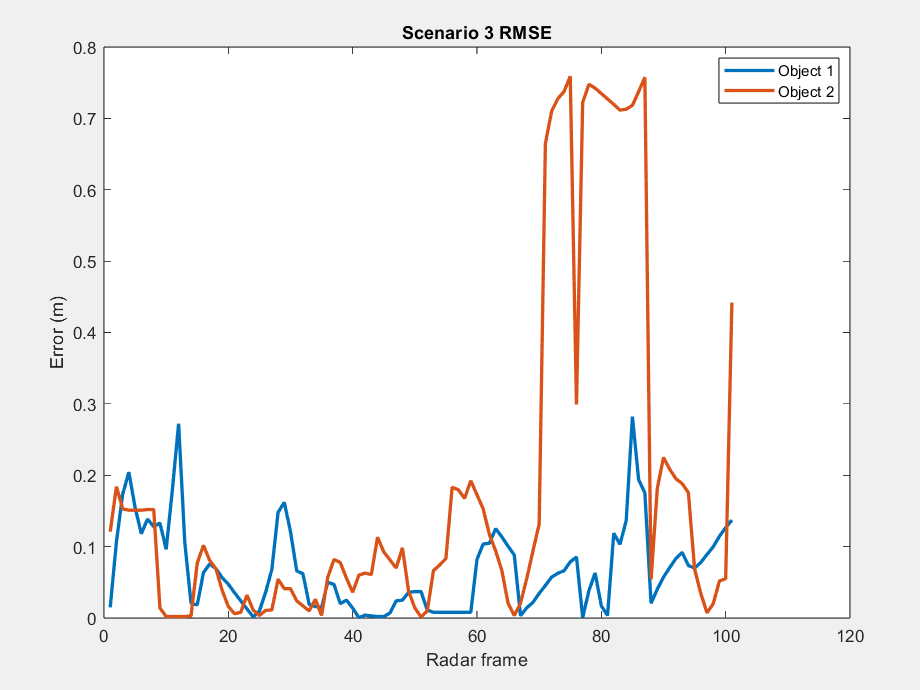
\includegraphics[width=7cm]{Figures/RMSE3.png}
        \caption{RMSE to ground truth}
        \label{subfig:RMSE_3}
    \end{subfigure}
    \caption{Scenario 3 multi-object tracking}
    \label{fig:scenario_result_3}
\end{figure}
\newpage
\subsection{Evaluation}\label{sec:3-evaluation}
\begin{table}[h!]
    \begin{center}
      \label{tab:table2}
      \begin{tabular}{c|c|c|c|c|c|c} % <-- Alignments: 1st column left, 2nd middle and 3rd right, with vertical lines in between
        \multirow{2}{*}{\textbf{Scenario}} & \multicolumn{3}{c|}{\textbf{Object 1}}  & \multicolumn{3}{c|}{\textbf{Object 2}}\\
        \cline{2-7}
                   & Fusion & Camera & Radar & Fusion & Camera & Radar \\
        \hline
        Scenario 1 & 0.1388 & 0.1922 & \textbf{0.1124} & \textbf{0.105}  & 0.1236 & 0.1201 \\
        Scenario 2 & \textbf{0.1206} & 0.1211 & 0.1228 & \textbf{0.1687} & 0.3728 & 0.2014 \\
        Scenario 3 & \textbf{0.0903} & 0.1211 & 0.0928 & 0.3075 & \textbf{0.2381} & 0.2487 \\
      \end{tabular}
    \end{center}
    \caption{All scenarios RMSE compared (m)}
    \label{tab:scenarios_rmse}
  \end{table}

  Which gives the average RMSE 0.1561m


  \begin{table}[h!]
    \begin{center}
      \label{tab:table1}
      \begin{tabular}{l|c|c|c|l} % <-- Alignments: 1st column left, 2nd middle and 3rd right, with vertical lines in between
        \textbf{Method} & \textbf{Radar} & \textbf{Object} & \textbf{Max Range} & \textbf{RMSE} \\% %object detected
        \hline
        Proposed & AWR1843 & human & 6m & 0.1561 m  \\%& 6m 
        \citeauthor{9081940}\cite{9081940} &  RT3002 & human & 40m & 0.18 m \\%
        \citeauthor{method1}\cite{method1} & AWR1642 & vehicle & 50m & 0.1828 m\\%& 50m
        \citeauthor{8932892}\cite{8932892} & IWR1443 & human & 6m & 0.2486 m\\%
        \citeauthor{8844649}\cite{8844649} & AWR1642 & human & 10m & 0.2902 m \\%
        
      \end{tabular}
    \end{center}
    \caption{Comparison of other tracking method}
    \label{tab:method_rmse}
  \end{table}


